\chapter{Metodologia}\label{cap:proposta}

Esta seção descreve a metodologia proposta para a tarefa de classificação da OA de joelho a partir de radiografias. A principal abordagem desta pesquisa consiste no uso de \textit{transfer learning} para aproveitar o conhecimento já obtido por modelos pré-treinados e melhorar a performance da predição final.

\section{Coleta de dados}

A seleção e coleta de dados constituem etapas iniciais fundamentais no desenvolvimento de modelos de aprendizado profundo. Nesse estudo, o conjunto de dados (ou \textit{dataset} do inglês) foi obtido por meio da plataforma Kaggle \citep{dataset-kaggle}, amplamente reconhecida por disponibilizar dados de alta qualidade e de acesso público para fins acadêmicos. O \textit{dataset} escolhido baseia-se na Osteoarthritis Initiative (OAI) e contém 9.786 radiografias de joelho rotuladas com suas respectivas classificações de severidade da OA, seguindo o sistema de Kellgren-Lawrence (\autoref{tabela-kl}). A escolha desta fonte deve-se à sua ampla utilização na plataforma e na literatura \citep{Tariq2023, Mohammed2023}, além do volume de imagens, fornecendo uma base sólida e representativa para o treinamento e avaliação dos modelos propostos. Um resumo do \textit{dataset} é apresentado na \autoref{dataset-summary}.

\begin{table}[ht]
    \centering
    \begin{tabular}{|c|c|c|c|}
        \hline
        \textbf{Classe KL} & \textbf{Descrição} & \textbf{Total de imagens} & \textbf{\% do total} \\
        \hline
        0 & saudável & 3857 & 40\% \\
        1 & duvidoso & 1770 & 18\% \\
        2 & mínimo & 2578 & 26\% \\
        3 & moderado & 1286 & 13\% \\
        4 & severo & 295 & 3\% \\
        \hline
        \textbf{Total} & - & 9786 & 100\% \\
        \hline
    \end{tabular}
    \caption{Número de radiografias por classe KL no conjunto de dados original.}
    \label{dataset-summary}
\end{table}

Todas as imagens possuem resolução de 224x224 pixels e estão no formato PNG. As imagens foram agrupadas em subconjuntos de treino, teste, validação e calibração, com uma proporção de 7:1:1:1. O conjunto de treino é utilizado para treinar os modelos, o conjunto de validação é usado para ajustar os hiperparâmetros e monitorar o desempenho do modelo durante o treinamento, o conjunto de teste é utilizado para avaliar o desempenho final do modelo e verificar sua capacidade de generalização em dados novos, e o conjunto de calibração é usado para aplicar a estratégia de predição conformal, discutida na \autoref{sec:conformal-prediction}. A distribuição das imagens por subconjunto de dados pode ser visualizada na \autoref{dataset-distribuition}.

\begin{figure}[ht]
    \centering
    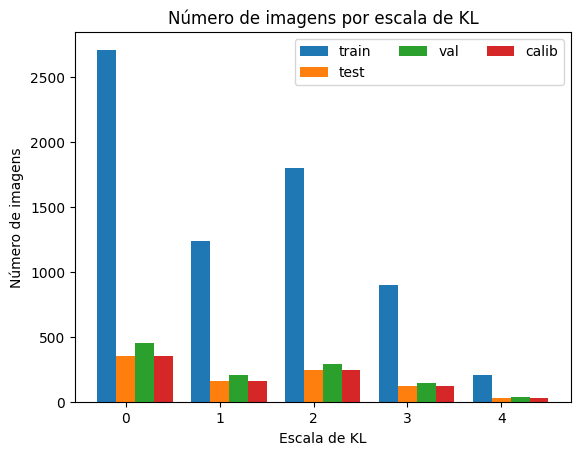
\includegraphics[width=0.7\linewidth]{figs/dataset-class-distribution.png}
    \caption{Distribuição das radiografias por classe KL nos subconjuntos de treino, teste, validação e calibração.}
    \label{dataset-distribuition}
\end{figure}

Com o objetivo de explorar diferentes abordagens para a classificação da severidade da OA de joelho, foram derivados, a partir do \textit{dataset} original contendo cinco classes, três novos conjuntos de dados: com 4, 3 e 2 classes. O conjunto com 4 classes foi construído por meio da exclusão da classe 1 (duvidosa), com a finalidade de simplificar o problema de classificação. O conjunto com 3 classes foi obtido pela remoção das classes 0 e 1 (respectivamente, saudável e duvidosa), resultando em um subconjunto composto apenas pelas instâncias que apresentavam algum grau de severidade (mínima, moderada ou severa). Por fim, o conjunto com 2 classes foi gerado ao se agrupar as classes 0 e 1, representando a ausência de OA, e as classes 2, 3 e 4, representando a presença de OA, formando, assim, um conjunto de dados binário.

\section{Pré-processamento das imagens}

A etapa de pré-processamento é essencial para garantir que as imagens estejam em um formato adequado para o treinamento dos modelos. Neste estudo, o pré-processamento das radiografias foi dividido em duas etapas: pré-processamento geral e pré-processamento específico para cada modelo. O pré-processamento geral, realizado antes do treinamento, inclui técnicas como equalização de histograma e filtro gaussiano. Já o pré-processamento específico para cada modelo, realizado durante o treinamento, envolve a adaptação das imagens às exigências de entrada dos modelos selecionados, como redimensionamento e normalização dos valores dos pixels. Além disso, o aumento de dados foi aplicado para expandir a variabilidade do conjunto de dados e mitigar o efeito do desbalanceamento entre as classes.

\subsection{Equalização de Histograma}

A equalização de histograma foi utilizada como técnica de pré-processamento com o intuito de melhorar o contraste das radiografias coletadas do conjunto original. Esse método redistribuiu os níveis de intensidade dos pixels de forma a abranger a maior faixa de valores possíveis, aumentando a separabilidade entre as regiões mais claras e mais escuras da radiografia. Em particular, essa técnica foi útil para realçar o contraste das estruturas ósseas e o espaço articular do joelho, assim como alterações ósseas sutis que podem ser indicativas de OA.

A aplicação da equalização de histograma foi realizada utilizando a biblioteca OpenCV \citep{opencv} do Python. A \autoref{fig:histogram-equalization}(a) ilustra uma radiografia original do joelho, enquanto a \autoref{fig:histogram-equalization}(b) mostra a mesma radiografia após a equalização de histograma. É possível observar que a equalização melhorou o contraste da imagem, tornando as estruturas ósseas mais visíveis. As respectivas distribuições de intensidade dos pixels antes e depois da equalização são apresentadas na \autoref{fig:histogram-equalization-histogram}.

\begin{figure}
    \centering
    \begin{tabular}{@{}c@{}}
        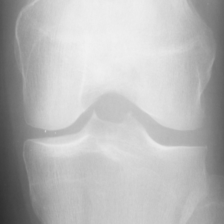
\includegraphics[width=0.45\textwidth]{figs/imagem-nao-equalizada.png} \\[\abovecaptionskip]
        \small (a) Radiografia original do joelho.
    \end{tabular}
    \hfill
    \begin{tabular}{@{}c@{}}
        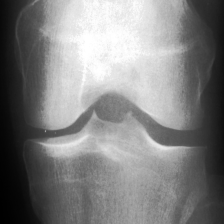
\includegraphics[width=0.45\textwidth]{figs/image-equalizada.png} \\[\abovecaptionskip]
        \small (b) Radiografia após equalização de histograma.
    \end{tabular}
    \caption{Exemplo de equalização de histograma aplicada a uma radiografia de joelho.}
    \label{fig:histogram-equalization}
\end{figure}

\begin{figure}
    \centering
    \begin{tabular}{@{}c@{}}
        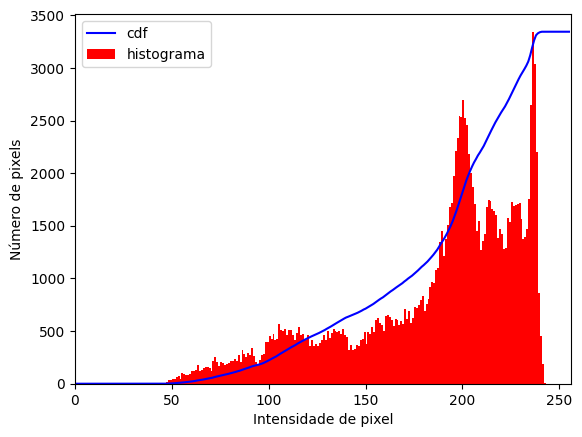
\includegraphics[width=0.45\textwidth]{figs/histograma-imagem-nao-equalizada.png} \\[\abovecaptionskip]
        \small (a) Histograma da radiografia original.
    \end{tabular}
    \hfill
    \begin{tabular}{@{}c@{}}
        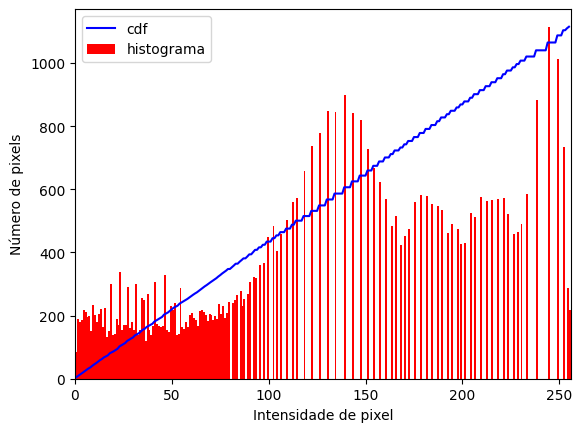
\includegraphics[width=0.45\textwidth]{figs/histograma-imagem-equalizada.png} \\[\abovecaptionskip]
        \small (b) Histograma da radiografia após equalização.
    \end{tabular}
    \caption{Distribuições de intensidade dos pixels antes e depois da equalização de histograma.}
    \label{fig:histogram-equalization-histogram}
\end{figure}

\subsection{Normalização}

A normalização das radiografias consistiu em uma etapa fundamental do pré-processamento, com o objetivo de padronizar a escala dos valores dos pixels e, assim, facilitar o aprendizado pelos modelos. Essa técnica foi aplicada convertendo os valores de intensidade dos pixels, originalmente na faixa de 0 a 255, para uma faixa padronizada entre 0 e 1.

Neste estudo, a normalização foi implementada em todos os subconjuntos de dados utilizando a função \texttt{transforms.Normalize} da biblioteca PyTorch \citep{pytorch}, que aplica a normalização em cada canal (RGB), subtraindo a média e dividindo pelo desvio padrão. Para modelos baseados em arquiteturas tradicionais, como ResNet e VGG, utilizaram-se os valores convencionais:

\begin{itemize}
    \item Média: 0.485, 0.456 e 0.406
    \item Desvio padrão: 0.229, 0.224 e 0.225
\end{itemize}

Para modelos baseados em ViTs, como o DeiT e o Swin Transformer, foram utilizados os valores de normalização específicos para esses modelos, obtidos diretamente do objeto \texttt{processor}, utilizando a função \texttt{processor.image\_mean} e \texttt{processor.image\_std}, garantindo a compatibilidade com o pré-processamento original desses modelos.

\subsection{Aumento de dados}

Com o objetivo de melhorar a generalização dos modelos e reduzir o risco de \textit{overfitting}, foi aplicado o aumento de dados (\textit{data augmentation}) nas radiografias durante o treinamento dos modelos.

A técnica consistiu na aplicação de transformações geométricas simples nas imagens do conjunto de treinamento, de forma a simular variações naturais que poderiam ocorrer nas radiografias. As transformações incluíram a inversão horizontal (reflexão), com probabilidade de 50\%, e rotações aleatórias limitadas a um intervalo de -10 a 10 graus.

Antes das transformações, as imagens foram redimensionadas para o tamanho esperado pelo modelo, definido como 224x224 pixels para todos os modelos, exceto para o modelo InceptionV3, que requer imagens de 299x299 pixels.

\subsection{Subamostragem}

Como pode ser observado na \autoref{dataset-summary}, o conjunto de dados original apresenta um desbalanceamento significativo entre as classes, com a classe 0 (saudável) representando 40\% do total de imagens e a classe 4 (severo) apenas 3\%. Para lidar com esse desbalanceamento, além do aumento de dados, foi aplicada a técnica de subamostragem (\textit{undersampling}) nas classes majoritárias e reduzindo o número de imagens dessas classes, equilibrando sua proporção em relação às classes minoritárias.

A subamostragem foi aplicada apenas no conjunto de treinamento, de modo a não comprometer a representatividade das distribuições no conjunto de validação, testes e calibração. A técnica consistiu na seleção aleatória de um subconjunto das amostras das classes até um limite definido de 1.700 imagens por classe. Esse limite foi escolhido com base na classe 2 (mínima), que possui o maior número de imagens entre as classes com severidade, garantindo que todas as classes fossem representadas de forma equilibrada no conjunto de treinamento.

Embora essa estratégia possa levar à perda de informações potencialmente úteis, ela ajuda a reduzir o viés do modelo em direção às classes majoritárias e melhora sua capacidade de aprender padrões relevantes em todas as classes.

\section{Treinamento dos modelos}

A técnica de \textit{transfer learning} foi aplicada no treinamento dos modelos de classificação da OA de joelho com o objetivo de reaproveitar os pesos dos modelos pré-treinados e acelear o processo de convergência. Esse processo envolveu o uso de modelos pré-treinados no conjunto de dados ImageNet 1K \citep{Russakovsky2015}, onde tais modelos foram treinados para classificar imagens em 1.000 categorias distintas. O uso deste método de treinamento foi especialmente útil para este estudo, pois o conjunto de dados de radiografias de joelho é limitado em tamanho, o que poderia dificultar a capacidade dos modelos de aprender padrões significativos nas imagens.

O processo de treinamento dos modelos foi conduzido segundo um protocolo padronizado, assegurando robustez e reprodutibilidade. As arquiteturas foram inicializadas com pesos pré‑treinados obtidos de repositórios conhecidos, como o \textit{PyTorch} e o \textit{Hugging Face}, e tiveram sua camada de saída ajustada para corresponder ao número de classes da tarefa específica (5, 4, 3 ou 2 classes) e ao exigido pela função de perda empregada, sendo que para a \textit{CORN} o número de classes da camada de saída é subtraído em uma unidade. Por fim, adotou‑se a estratégia na qual todas as camadas da rede permaneceram treináveis. A última escolha foi motivada pela melhoria que essa abordagem pode proporcionar, embora aumente o tempo de treinamento.

Cada modelo foi treinado com um \textit{batch size} de 28 imagens durante 60 épocas, utilizando uma política de embaralhamento aleatório dos dados. O otimizador Adam foi selecionado, com uma taxa de aprendizado inicial de 0,0001, e um \textit{scheduler} para diminuir a taxa de aprendizado em um fator de 10 a cada 5 épocas. Além disso, foi implementado um mecanismo de parada antecipada, com paciência de 5 épocas, baseado na perda de validação, para evitar o \textit{overfitting} dos modelos. A cada época, registraram‑se as métricas de desempenho em treinamento e validação; a taxa de aprendizado foi reduzida em ordem de magnitude a intervalos pré‑definidos, e o modelo de melhor acurácia de validação foi preservado.

Concluído o treinamento, obteve-se os pesos do melhor modelo e traçaram‑se curvas de desempenho para análise visual da convergência. A avaliação final foi conduzida no conjunto de teste, produzindo o relatório de métricas de classificação descrita na \autoref{sec:avaliacao-metricas}. A complexidade computacional de cada arquitetura, em termos de FLOPs e quantidade de parâmetros, foi estimada com auxílio da bibliteca \texttt{ptflops} \citep{ptflops}. Todos os resultados, incluindo métricas, tempo de execução e medidas de complexidade, foram armazenados em formato JSON para análise posterior.

Todos os modelos foram treinados no ambiente de computação em nuvem Google Colab, utilizando uma Nvidia T4 GPU com 16 GB de memória, adequada para a tarefa de ajuste fino em modelos pequenos. A escolha dessa plataforma foi motivada pela sua acessibilidade e capacidade de fornecer recursos computacionais adequados a um custo reduzido. A seguir, são apresentados os experimentos realizados com cada modelo, incluindo as métricas de desempenho obtidas e a análise dos resultados.

\section{Experimentos}

Os modelos de classificação foram treinados e avaliados em diferentes cenários, variando o número de classes e a função de perda utilizada, com o objetivo de analisar o impacto dessas variáveis no desempenho dos modelos. A seguir, são apresentados os cenários de experimentos realizados:

\subsection{Número de classes}

Os modelos foram treinados em quatro cenários distintos, variando o número de classes na camada de saída:

\begin{itemize}
    \item \textbf{5 classes}: O cenário original, com as classes 0 (saudável), 1 (duvidosa), 2 (mínima), 3 (moderada) e 4 (severa).
    \item \textbf{4 classes}: Cenário com a exclusão da classe 1 (duvidosa), resultando nas classes 0 (saudável), 2 (mínima), 3 (moderada) e 4 (severa). Esse cenário foi escolhido devido à dificuldade de classificar a classe 1, que muitas vezes é considerada ambígua ou de difícil distinção entre saudável e mínima.
    \item \textbf{3 classes}: Cenário com a exclusão das classes 0 (saudável) e 1 (duvidosa), resultando nas classes 2 (mínima), 3 (moderada) e 4 (severa), que representam apenas os casos de OA de joelho com algum grau de severidade.
    \item \textbf{2 classes}: Cenário binário, onde as classes 0 (saudável) e 1 (duvidosa) foram agrupadas em uma única classe, representando a ausência de OA, enquanto as classes 2 (mínima), 3 (moderada) e 4 (severa) foram agrupadas em outra classe, representando a presença de OA.
\end{itemize}

\subsection{Função de perda}

Além da variação no número de classes, os modelos foram treinados utilizando duas funções de perda distintas:

\begin{itemize}
    \item \textbf{Cross-Entropy}: A função de perda padrão para problemas de classificação multiclasse, que mede a discrepância entre as distribuições de probabilidade previstas e as reais. É uma opção comum, mas não leva em consideração a característica ordinal das classes.
    \item \textbf{CORN}: Uma função de perda adaptada para problemas de classificação ordinal, que considera a ordem das classes e penaliza erros de classificação com base na distância ordinal entre as classes.
\end{itemize}

\section{Avaliação e Análise Complementar}

Além das métricas de classificação padrão, foram realizadas análises complementares para avaliar a incerteza, a eficiência e a interpretabilidade dos modelos.

\subsection{Predição Conformal}

Para quantificar a incerteza associada às previsões dos modelos, este estudo empregou a técnica de predição conformal. Diferentemente de uma predição única, a predição conformal fornece um conjunto de classes que contém a classe verdadeira com uma alta probabilidade, analisando uma nova amostra e respondendo algo como ``Esta radiografia é classificada com nível de osteoartrie de joelho 2 com 95\% de confiança''. Essa abordagem é particularmente útil em cenários médicos, onde a incerteza pode ter implicações significativas para o diagnóstico e tratamento.

A predição conformal foi aplicada utilizando o conjunto de calibração, previamente separado com 10\% das imagens do conjunto de dados original, com um valor de confiança de 95\% ($\epsilon = 0.05$). Para modelos treinados com a função de perda \textit{cross-entropy}, o limiar de confiança $\hat{q}$ foi calculado seguindo a abordagem descrita na \autoref{sec:conformal-prediction}, onde os \textit{scores} foram obtidos a partir das previsões do modelo. No entanto, para modelos treinados com o CORN, seguir a abordagem tradicional não é viável, pois seria necessário reconstruir explicitamente as probabilidades por classe. Em vez disso, foi adotada uma abordagem alternativa, tratando como conjunto de tarefas binárias ordenadas, que é exatamente como o CORN opera. Assim, para um problema com $K$ classes KL, a predição conformal foi aplicada por limiar, da seguinte forma:

\begin{itemize}
    \item Para cada exemplo do conjunto de calibração:
    \begin{itemize}
        \item Para cada limiar $k \in \lbrace 0 \text{, } ... \text{, } K-2 \rbrace$:
            \begin{itemize}
                \item Se $y_{\text{true}} > k$, $\text{score} = 1 - p$, onde $p$ é a probabilidade prevista pelo modelo para o limiar $k$.
                \item Se $y_{\text{true}} \leq k$, $\text{score} = p$.
            \end{itemize}
    \end{itemize}
    \item Calcular o limiar de confiança $\hat{q}_i$ para cada limiar do problema $k$ da mesma forma que na abordagem tradicional.
    \item Durante a inferência:
        \begin{itemize}
            \item Para cada limiar $k$, adicione a classe $k+1$ ao intervalo de predição se $1 - p_k \leq \hat{q}_k$.
        \end{itemize}
    \item Construir a predição ordinal intervalar:
        \begin{itemize}
            \item Exemplo: $\hat{y} \in [0,2]$ se apenas $k_0$ e $k_1$ estiverem acima do limiar de confiança.
        \end{itemize}
\end{itemize}

\subsection{Análise do Tempo de Inferência}

Para avaliar a viabilidade prática dos modelos em cenários de aplicação real, além da complexidade teórica (FLOPs), foi mensurado o tempo de inferência. Para cada modelo treinado, o tempo necessário para realizar uma predição em uma nova radiografia foi registrado. A fim de garantir uma medida robusta e estável, o \textit{script} de inferência foi executado 50 vezes para cada modelo, e a média dos tempos foi calculada e registrada. Essa análise é fundamental para comparar a eficiência computacional prática das diferentes arquiteturas.

\subsection{Análise de Interpretabilidade com Grad-CAM}

Para entender e interpretar as decisões dos modelos, foi utilizada a técnica de visualização Grad-CAM (Gradient-weighted Class Activation Mapping). Essa abordagem gera mapas de calor que destacam as regiões da radiografia que foram mais influentes para a predição de uma determinada classe. Foram geradas e registradas imagens Grad-CAM para todos os modelos treinados. O objetivo dessa análise foi inspecionar visualmente se os modelos estavam focando em regiões clinicamente relevantes, como o espaço articular e a formação de osteófitos, e comparar os padrões de ativação entre as diferentes arquiteturas.